\documentclass[10pt,a4paper]{report}
\usepackage[utf8]{inputenc}
\usepackage[T1]{fontenc}
\usepackage{graphicx}
\usepackage{amsmath}
\usepackage{float}
\usepackage{xfrac}
\usepackage[toc]{glossaries}
\usepackage[font=footnotesize]{caption}
\usepackage[toc,page]{appendix}
\usepackage[pdfpagelabels]{hyperref}
\setlength{\parskip}{1em}

\newacronym{fpga}{FPGA}{Field-programmable gate array}
\newacronym{gui}{GUI}{Graphical User Interface}
\newacronym{wav}{WAV}{Waveform Audio File Format, also referred as WAVE}
\newacronym{dft}{DFT}{Discrete Fourier Transform}
\newacronym{dfft}{DFFT}{Discrete Fast Fourier Transform}
\newacronym{ntsc}{NTSC}{National Television System Committee}
\newacronym{dbfs}{dBFS}{Decibels relative to full scale}
\newacronym{png}{PNG}{Portable Network Graphic}
\newacronym{hz}{Hz}{Hertz is the derived unit of frequency in the International System of Units (SI). It is defined as one cycle per second.}
\newacronym{khz}{kHz}{Kilohertz, refers to 1000 hertz.}

\newcommand{\define}[1] {
	\textit{\acrshort{#1}\footnote{\textit{\acrlong{#1}}}}}

\newcommand{\defineCite}[2] {
	\textit{\acrshort{#1}\footnote{\textit{\acrlong{#1}} #2}}}

\makeglossaries

%opening
\title{MDFourier}
\author{Artemio Urbina}

\begin{document}
	
\pagenumbering{Alph}
\begin{titlepage}
	\maketitle
	\thispagestyle{empty}
\end{titlepage}
\pagenumbering{arabic}

\begin{abstract}
\textit{MDFourier} is a \textit{open source} software created to compare \textit{audio signatures} and generate a series of graphs that show how they differ. The software consists of two separate programs, one that generates the signal for recording from the console and the other that analyses and displays the audio comparisons. 

The information gathered from the comparison results can be used in a variety of ways: to identify how \textit{audio signatures} vary between \textit{systems}, to detect if the \textit{audio signals} are modified by \textit{audio equipment}, detect if \textit{modifications} resulted in audible changes, to help tune \textit{emulators}, \textit{FPGA} implementations or \textit{mods}, etc.

This document serves as an introduction, a manual and description of the methods used and how they work. Its intent is to guide new users in making simple comparisons while still providing advanced users with information to perform a more detailed analysis of audio signatures.
\end{abstract}

\tableofcontents

\chapter{\textit{MDFourier} Objective}

To provide a free and open source\footnote{Licensed under \textit{GNU GPL} see appendix \ref{license}.} software based analysis framework for comparing audio signatures from a targeted video game system and its variants\footnote{Vintage retail variations, hardware modifications, clones and \textit{\acrfull{fpga}} implementations}. The resulting comparison can help tune such system\footnote{The term \textit{system} will be used to cover vintage retail hardware, emulators, \textit{FPGA} implementations and any other possible variant that executes binaries for the target hardware} to better match the desired reference profile.

This is of course not limited to one specific system, and the software can be used to compare any other platform with new configuration files\footnote{At the moment a profile for \textit{Mega Drive/Genesis} is functional and implemented with more to follow.}.

The intention is not to disparage any particular system; but to help understand and improve them whenever possible by identifying their differences.

A secondary but not less important goal is to create a community driven catalog of audio signatures from these systems, in order to help preservation efforts achieve their objectives.


\section{What is it for?}

\textit{MDFourier} can be used to identify the differences between two audio signatures. For instance a \textit{Sega Genesis Model 1 VA3} and a \textit{Sega Genesis Model 2 VA 1.8}\footnote{These two models are typically listed as having notorious audio differences \cite{genesisaudio}} can be compared in order to verify how different they are across the audible spectrum. 

It can also be used to compare a vintage version of the console against any other variation, like an emulator or an \textit{FPGA} implementation.

Another possible application is to determine if there were changes in the audio spectrum after modifications to a console, like recapping or changing the audio circuitry.

These results can help determine if the signals are indeed different, and how they differ across the human hearing frequency spectrum. Such information can then be used for different means, such as recreating specific audio signatures, tuning to a different taste, etc; based on an objective, repeatable and measurable data set provided by the framework.

It can also be used to evaluate if equipment - such as switchers and upscalers with audio passthrough - have any effect on the signal, by comparing a recording with and without the device connected in the AV\footnote{Audio/Video} chain.

Although I believe any present and future implementation of a gaming platform should offer a configuration based on vintage retail hardware, that doesn't mean there isn't room for improvement upon those configurations. Reducing noise while keeping the reference sound signature is one such case.

There must be powerful industrial solutions for this kind of analysis, but they do not seem to have reached the enthusiast for this purpose. I'm not aware of any other similar effort to create public software analysis tools\footnote{It must be noted that there have been detailed comparisons made in particular for the \textit{MegaDrive/Sega Genesis}, see post at \cite{genesisaudio}} that are aimed at vintage console hardware. 

\newpage
\section{Disclaimer}

\textit{MDFourier} is a work in progress, just as the current document. It still has a few rough edges, and although I tried to adhere to the best practices known to me, my expertise in \textit{digital signal processing} was almost non-existent before this project. 

If you have suggestions, please contact me. Any corrections and improvements are encouraged and welcome. Contact information is available in appendix \ref{contact}.

This project was born from my curiosity to compare the audio signatures of different revisions of the  \textit{Mega Drive/Genesis}, and verify them with a tool assisted analysis. I was also curious about \textit{FPGA} and software implementations, and how similar they were to vintage console audio signatures.

\chapter{How \textit{MDFourier} works}
\label{howitworks}

The first thing to keep in mind is what \textit{MDFourier} does. It takes two signals, the first one is the \textit{Reference} file and the second one is the \textit{Comparison} file.

The \textit{Reference} file is used as a control. This means that its characteristics are considered the true values to be expected and against which the \textit{Comparison} file will be evaluated. In consequence, all results are relative between the signals.

These files are audio recordings from the desired hardware, preferably captured with a flat frequency\footnote{Flat frequency response refers to the capability of capturing the whole audible spectrum with little or no variation, regardless of frequency. A non flat frequency card can be used to gather relative information, but the captures won't match the ongoing catalogue in order to make further comparisons.} audio capture card\footnote{See \textit{Audio Cards} in appendix \ref{requirements}} and generated by a \textit{custom binary}. This \textit{custom binary} is targeted for the particular hardware capabilities and frequency range. Whenever possible, this binary will be part of the \textit{240p Test Suite}\footnote{A homebrew software suite for video game consoles developed to help in the evaluation of TVs, upscalers, upscan converters, line doublers and video processing in general.\cite{240pSuite}}. 

The analysis software is itself \textit{command line} based, in order to be multi-platform and offer it on every operating system that has an \textit{C compiler}\footnote{\textit{ANSI C99 compiler}}. However a \define{gui} front end for \textit{Microsoft Windows} is provided for simplicity and accessibility. Not all options from the command line tool are present via the \textit{GUI}, but the most relevant ones are readily available. Full Source code can be downloaded from \textit{github} \footnote{See download link \cite{sourcecode}}.

\section{File alignment}

\textit{MDFourier} takes both files and auto detects the starting and ending point of the recording. These are identified by a series of \textit{8820}\define{hz} pulses in the current \textit{Mega Drive/Genesis} implementation. From these, a \textit{frame rate}\footnote{The \textit{frame rate} is the ratio at which the console sends video frames to a display. For more details see appendix \ref{framerate}} is calculated in order to trim each file\footnote{Since audio cards have their own \textit{sample rate} clocks \cite{SoundCardClock} \cite{soundcardtiming} \cite{gwsoundcardtiming}, and some implementations have different \textit{frame rates}, frames are used as the base unit instead of time codes} into the segments that are defined in the \textit{configuration file}\footnote{This file specifies the operating parameters for each hardware configuration. It is described in appendix \ref{mfnconfig}} for further comparison.

Most importantly, it guarantees that the \textit{Reference} and \textit{Comparison} files are logically aligned, and that each note - or segment - is compared to its corresponding one, with no overlap and without any audio editing or trimming skills required from the user. Current pulse detection accuracy is around $\sfrac{1}{4}$ of a millisecond.

After alignment is accomplished, the software reports the starting and end points of both signals, in seconds and bytes.

\section{The heart of the process}

In order to compare the signals, audio levels are checked and a relative \textit{normalization}\footnote{This process is detailed in appendix \ref{normalization}} takes place, based on the maximum amplitude of the \textit{Reference} file. A local maximum search is done in the same frame on the \textit{Comparison} signal, and that amplitude is then used to normalize both files. This is done in the \textit{frequency domain}, in order to reduce amplitude imprecision when comparing recordings with different \textit{frame rates}. The software does have the option to do this in the time domain, but quantization and amplitude imprecision is to be expected in such case.

Then a \textit{Discrete Fourier Transform}\footnote{\gls{dft} is the variant of \textit{Fourier Transform} applied to discrete values, such as the ones we have in the audio file \cite{FourierTransformApps}} is used in order to analyze the frequency content of the signal, as well as the amplitudes from each of the corresponding fundamental frequencies that compose the audio signal.

The software uses the \textit{FFTW}\footnote{\textit{The Fastest Fourier Transform in the West} \cite{fftw}} library in order to accomplish this, and then proceeds to sort out the frequencies of each block by amplitude. It can be configured to compare a range of these frequencies, but by default it compares 2000 of them for each element defined in the \textit{mfn} configuration file\footnote{Described in appendix \ref{mfnconfig})}.

I've found such comparison to be more than enough, and the \textit{minimum significant volume}\footnote{See section \ref{MinSigVolume}} even limits these 2000 to a lower number, based on significant amplitude\footnote{The terms \textit{volume} and \textit{amplitude} are used interchangeably during the document, however they are technically not the same thing. \textit{Volume} refers to the perception of \textit{loudness}, and \textit{amplitude} is the \textit{quantifiable} quality of the signal related to its power. As a result, the software can only use amplitude for its calculations.}. In case more frequencies are needed, this can be changed via a command line parameter.

After comparing these frequencies between both files, matches are made and the differences in volume are plotted to a graph. Please read chapter \ref{howtoplots} to help you understand the various plots created by this program.

Sometimes it is helpful to listen to the results of these limiting filters, in order to evaluate if - for instance - 2000 frequencies are either enough or too little for the current application. For this and other purposes I made an extra tool named \textit{MDWave}\footnote{Described in appendix \ref{mdwave}}, which creates segmented audio files as internally processed by \textit{MDFourier}, even including the effects of \textit{window}\footnote{Window functions are described in section \ref{windows})} filters and amplitude limits.

If you are interested in learning what the \textit{Fourier Transform} does and how it works it's magic, there are several resources online to help you out. Here are a few:

\begin{itemize}
	\item But what is the Fourier Transform? A visual introduction.\\ \url{https://www.youtube.com/watch?v=spUNpyF58BY}
	\item An Interactive Introduction to Fourier Transforms.\\ \url{http://www.jezzamon.com/fourier/}
	\item The Uncertainty Principle and Waves.\\
	\url{https://www.youtube.com/watch?v=VwGyqJMPmvE}
\end{itemize}

\section{Minimal significant volume}
\label{MinSigVolume}

Although the whole frequency spectrum can be compared, there is little practical use in doing so -  due to execution time and extra noise from low amplitude harmonics. As a result, rule of thumb defaults are set in order to minimize these issues.

One of these values is a \textit{minimum volume} at which to stop comparing the fundamental frequencies that are found after decomposing the signal with the \textit{Fourier Transform}. This is the \textit{minimal significant volume} and it is the cutoff at which comparisons made by the software are stopped.

This volume is the \textit{amplitude}, and it is measured in \define{dbfs}. In the \textit{dBFS} scale, the value of \textit{0} is assigned to the maximum possible digital level and it can go down to $-\infty$.\footnote{The minimum volume when using \textit{16 bit} samples is -96dBFS.}

Currently \textit{MDFourier} can recognize three scenarios to define the \textit{minimum significant volume} to compare the signals, and the three are derived from the first \textit{silence block} in the file.

The first scenario is the grid power frequency noise, which currently searches for \textit{60/50hz} noise\footnote{\textit{PAL} needs to be tested yet, since I don't have console for that video system}. 

The second one is \textit{refresh rate noise}, again derived from the frame rate, in \textit{NTSC} it is around \textit{15697-15698hz}. 

If neither is found, which would be surprising for a file generated by recording from a vintage console via analogue means, the frequency with the highest volume within the silence block is used. 

Finally, in case none of the previous scenarios is met - or if those values are lower than \textit{-60}\textit{dbfs} - a default level of \textit{-60dBFS}\footnote{This can be changed via \textit{command line} options if needed.} is used. 

\section{Workflow}

The first step is loading the custom binary to your console, this varies from a \textit{flash cart}, burning a \textit{CD-ROM} or using a \textit{custom loader}.

The next step is setting up your \textit{audio capture card} and computer, in order to record a \textit{44 or 48\define{khz} 16 bit stereo} \define{wav} file\footnote{At the moment only 16 bit WAV files with PCM encoding and at 44.1 or 48kHz are supported. In the future \textit{FLAC} support could be added to save space and bandwidth. \textit{MP3} is not supported since it alters the results in this type of analysis, as shown in section \ref{mp3}}.

Once the \textit{capture card} is ready and the cables are hooked up from the console to the \textit{capture card}, start recording on the computer and execute the \textit{MDFourier} test from the console.

Wait for the console to show a message indicating you can stop recording, this typically takes less than 1 minute. After you have at least two files: a \textit{reference} - which can be one of the provided files -  and a \textit{comparison} file, you are ready to go. 

\chapter{How to use the Front End}
\label{usinggui}
The current version of the front end allows access to the main options of \textit{MDFourier}. It is a \textit{Windows} executable and all corresponding files must be placed in the same folder. \textit{Uncompressing} the package to a folder should have all that is necessary to run the program.

After executing \textit{MDFourierGUI.exe} you should be presented with the following interface:

\begin{figure}[H]
	\centering
	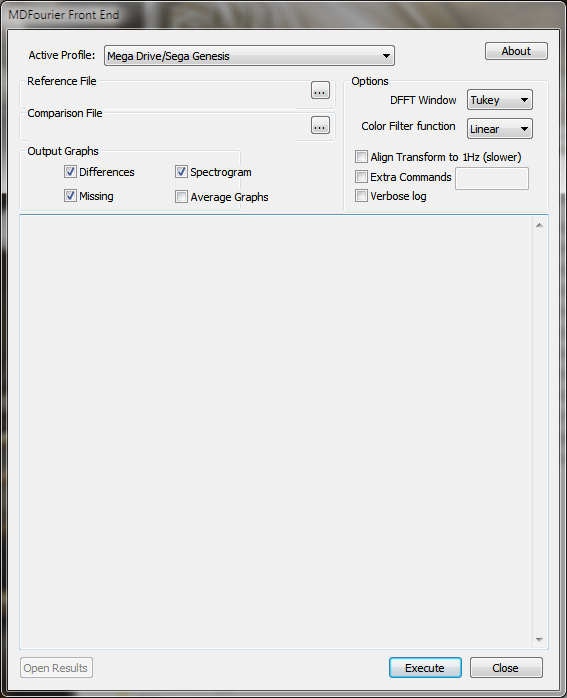
\includegraphics[width=0.6\linewidth]{images/GUI/GUI1.png}
	\caption[Front End]{MDFourier Windows Front End}
	\label{fig:gui1}
\end{figure}

In order to generate the output plots, two files must be selected to compare them. One as a \textit{Reference} and the other as the \textit{Comparison} file, as detailed in section \ref{howitworks}.

The following sequence of steps indicates the typical work flow within the GUI:

\begin{figure}[H]
	\centering
	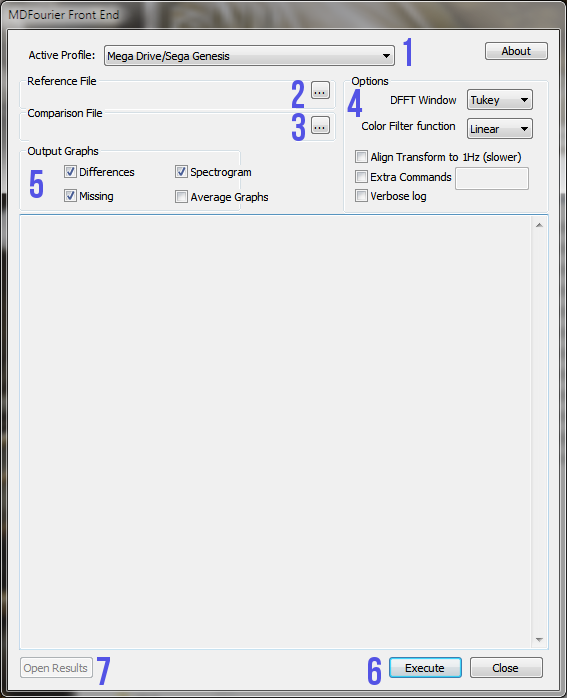
\includegraphics[width=0.6\linewidth]{images/GUI/GUI2.png}
	\caption[Steps]{Typical sequence of steps}
	\label{fig:gui2}
\end{figure}

\begin{enumerate}
	\item Select a \textit{Reference} file
	\item Select a \textit{Comparison} file
	\item Change the default \textit{options} if needed
	\item Select the desired output \textit{plots}
	\item Execute \textit{MDFourier}
	\item When execution ends, open the \textit{results folder}
\end{enumerate}

The \textit{Front End} will display the output text from the command line tool, including any errors or progress as it becomes available.

Keep in mind that the \textit{Open Results} button will only be enabled after a successful comparison between files has finished, and it won't open a second instance of the window if you have one already present.

The default options will generate plots that work on most situations. In some cases fine tuning the results might highlight specific aspects. These options will be described in the following sections.

\section{Front End Options}

The currently available options in the \textit{Front End} are:

\subsection{Window Functions}
\label{windows}

In order to reduce \textit{spectral leakage}\footnote{This term describes new frequency components created when applying a Fourier Transform to a segment of a signal. See \cite{leakage}} when applying the \define{dft} a \textit{filtering window}\footnote{All details regarding the windows used, their formulas and graphs are in appendix \ref{windowfunctiondetails}} is applied to each element to be compared between both signals. Since we are generating the signal ourselves from the \textit{custom binary}, the signal can be analyzed as \textit{periodic}\footnote{In theory this means we could get away without applying a window, but in practice the signal is not perfect and \textit{windowing} the data helps to eliminate noise.}, and has a natural \textit{attack} and \textit{decay} rate if possible.

By default we use a custom \textit{Tukey window}\footnote{This is not a common choice for window function, but was selected due to the above reasons after comparing results with  the rest of the available options.} with very steep slopes. \textit{MDFourier} does offer alternate windows as options for further analysis.

\subsection{Color Filter Functions}
\label{colorfilter}

Each dot in the \textit{Differences} graph uses the \textit{X axis} for the frequency range and the \textit{Y axis} for the amplitude difference between the \textit{Comparison} and \textit{Reference} signals.\footnote{See section \ref{outputfiles} for output file details}

Color intensity of each dot is used to represent the amplitude for that frequency in the \textit{Reference} signal. In other words, how relevant it was to create the original signal in that note. Please refer to chapter \ref{howtoplots} in order to see examples of their use.

A color scale is presented in each graph, with the color graduation and the corresponding volume level.

\begin{figure}[H]
	\centering
	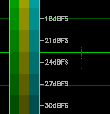
\includegraphics[width=0.2\linewidth]{images/colorfilter/colorscale.png}
	\caption[Plot color scale]{Detail of color scale in plot}
	\label{fig:colorscale}
\end{figure}

The options are useful to \textit{highlight} or \textit{attenuate} these differences by applying the range to one of the following functions. 

They are sorted in descending order. The topmost option will highlight all differences; and the bottom one will attenuate most of them, and show just the ones with highest amplitudes in the \textit{Reference} signal.

All filters, their graphs and effects are listed in appendix \ref{filterfunctions}.

\subsection{Align Transform to 1hz}

When designing the \textit{audio signal} for use during analysis, one consideration is how to balance gathering more information versus the duration of each recording. 

For practical reasons, it is desirable to have a short test that will be recorded for analysis. This reduces the time it takes to digitize audio from several systems, the storage used, analysis time by the software, and makes distributing such files easier.

In contrast, when applying the \textit{Fourier transform} a compromise is made between frequency detail and time accuracy, very similar to the Heisenberg's uncertainty principle. If we compare a longer signal for each element, we end up with more frequency information. In our case, we don't care much about time accuracy but we do care about the length of the test. Nobody wants to record a 5 or 10 minute signal for each test to be made.

The compromise made is to use \textit{sub second signals} for each element to be compared. Since the time and sample rate determine how the \textit{DFT} \textit{frequency bins}\footnote{The size of each slice in hz for the frequency spectrum} are spaced after analysis - and how much information we end up analyzing - the end result is a lower plot resolution.

Zero padding the input signal for Fourier analysis is a controversial subject\footnote{Zero-padding a signal does not reveal more information about the spectrum. See \cite{zeropaddinginterpolate} \cite{ZeroPaddingBad}}, but for the present application no adverse effects have been found. This might be the case since we control how the source signal is generated, with a predetermined \textit{attack} and \textit{decay}. However, it is disabled by default so the results presented can be free from questioning regarding the effects, and available for cases where more precise frequency information is needed with no spectral leakage to adjacent \textit{frequency bins}.

\subsection{Output Plots}
\label{outputfiles}

Several plots will be generated as a result of the analysis. There will be several plots of each type in the \textit{output folder}\footnote{It is named \textit{MDFourier} and a subfolder named as the compared files. It can be accessed from the \textit{Front End} with the \textit{Open Results} button.}. One for each type, and one that summarizes all types in a single plot.

All plots are saved in the \defineCite{png}{support via \textit{libpng} \cite{libpng}} format, which is lossless and open source. Please read section \ref{howtoplots} for examples and a guide to interpret their meaning. 

\subsubsection{Different Amplitudes}

Enabling this option created the most relevant output plots from \textit{MDFouriuer}. These contain the amplitude difference for the frequencies common to both files across the hearing spectrum using the \textit{Reference} file as control.

If the files are identical, the plot will be a perfect line across the \textit{0 dBFS} line. In case the signals differ, a scatter plot will show how it behaves across the typical human hearing spectrum\footnote{Typically defined as \textit{20-20000hz}, but the higher end tends to be lost with age.}.

The file names for these plots have the format:\\ \textit{DA\_Reference\_vs\_Comparison\_block\_options.png}

\subsubsection{Missing Frequencies} 

Plots the frequencies available in the \textit{Reference} file but not found in the \textit{Comparison} file within the significant amplitude range. This is in effect a \textit{Spectrogram}, but limited to the frequencies that were expected to be in the intersection but that were not present in the \textit{Comparison} file.

The file names for these plots have the format:\\ \textit{MIS\_Reference\_vs\_Comparison\_block\_options.png}

\subsubsection{Average Plot}
\label{averaged}

This option traces an \textit{average line} on top of the \textit{Difference} plots, making it easier to follow the trend when the output has severely scattered data. It is \textit{off by default}.
 
The curve is created by averaging time segments from the frequency data sorted in ascending order. A \textit{Simple Moving Average}\footnote{This is a type of average that is intended to smooth out sudden peaks in the data. Often used in exchange rate plots. See \cite{sma}.} is then calculated to smooth out the results.

The curve is weighted according to the \textit{Color Filter Functions} described in section \ref{colorfilter}, by a repeating each data point by the amount mapped in the \textit{0-1} interval described by the function.

As a result, the average will follow the relative amplitudes from the \textit{Reference} signal proportional to the selected \textit{filter function}.

If there is need for a plot without weighting, please disable the \textit{Color Filtering function}.

The file names for these plots have the format:\\ \textit{DA\_AVG\_Reference\_vs\_Comparison\_block\_options.png}

\subsubsection{Spectrograms}

Plots all the frequencies available in each file\footnote{As limited by the analysis parameters, such as amplitude and frequency count per block}. Two sets of spectrograms are generated, one for the \textit{Reference} file and one for the \textit{Comparison} file.

The file names for these plots have the format:\\ \textit{SP\_AVG\_Reference\_vs\_Comparison\_block\_options.png}

\subsection{Extra Command}
\label{extracommand}

This checkbox enables the text field to send any extra commands that are not available via the GUI to \textit{MDFourier}. 

Current options as of version \textit{0.918} are:

\begin{verbatim}
MDFourier 0.918 [240p Test Suite Fourier Audio compare tool]
Artemio Urbina 2019 free software under GPL

usage: mdfourier -r reference.wav -c compare.wav
FFT and Analysis options:
-a: select <a>udio channel to compare. 's', 'l' or 'r'
-w: enable <w>indowing. Default is a custom Tukey window.
'n' none, 't' Tukey, 'h' Hann, 'f' FlatTop & 'm' Hamming
-f: Change the number of analyzed frequencies to use from FFTW
-s: Defines <s>tart of the frequency range to compare with FFT
-e: Defines <e>nd of the frequency range to compare with FFT
-i: <i>gnores the silence block noise floor if present
-t: Defines the <t>olerance when comparing amplitudes in dBFS
-z: Uses <z>ero Padding to equal 1 hz FFT bins
-n: <N>ormalize: 't' Time Domain Max, 'f' Frequency Domain Max or 'a' Average
-B: Do not do stereo channel audio <B>alancing
Output options:
-l: <l>og output to file [reference]_vs_[compare].txt
-v: Enable <v>erbose mode, spits all the FFTW results
-g: Create avera<g>e points over the plotted graphs
-A: Do not weight values in <A>veraged Plot (implies -g)
-L: Create 800x400 plots as shown in the manual
-H: Create 1920x1080 plots
-D: Don't create <D>ifferences Plots
-M: Don't create <M>issing Plots
-S: Don't create <S>pectrogram Plots
-d: Max <d>BFS for plots vertically
-k: cloc<k> FFTW operations
-j: (text) Cuts per block information and shows <j>ust total results
-x: (text) Enables e<x>tended log results. Shows a table with all matches
-m: (text) Enables Show all blocks compared with <m>atched frequencies
-h: Shows command line help
\end{verbatim}

Sending \textit{-h} in this field will enlist all the currently supported options for your version.

\subsection{Verbose Log}
\label{verbose}

A log is always created by default when using the \textit{Font End}, however this option enables a verbose version with the whole frequency analysis and many other details dumped to the file. 

Useful for reporting errors or unexpected behavior. \textit{Please send the audio files if possible as well!}\footnote{Contact details are available in appendix \ref{contact}.}

\chapter{How to interpret the plots}
\label{howtoplots}

The main output of the program is a set of different graphics that vary in quantity based on the definitions made in the \textit{mfn} file detailed in appendix \ref{mfnconfig}.

In its current form for the \textit{Mega Drive/Genesis}, there are three \textit{active blocks}\footnote{\textit{The Mega Drive/Sega Genesis} has two audio synthesizers: a \textit{Yamaha 2612} (YM2612) for \textit{Frequency Modulated} (FM) audio, and a \textit{Texas Instruments SN76489 Programmable Sound Generator} (PSG)  - or equivalent in an \textit{ASIC} - for \textit{Sega Master System} compatibility and extra audio channels. }: \textit{FM}, \textit{PSG} and \textit{Noise}. These will result in a plot of each type, and a general plot, being generated as output.

The files are saved under the folder \textit{MDFourier} and a sub-folder named after the input \textit{WAV} file names. They are stored in \textit{PNG} format, currently \textit{1600x800} plots are used, although this can be changed via options. 

For the current document \textit{800x400} plots were used in order to fit within a \textit{PDF} or \textit{HTML} presentation. The output plots that are created by the software are listed and described in section \ref{outputfiles}.

In our current \textit{Mega Drive/Genesis} scenario and with default options enabled, we'll get four plots of each type: \textit{FM}, \textit{PSG}, \textit{Noise} and a general one, named \textit{ALL}.

We'll follow a series of results from different input files to \textit{MDFourier}, starting with cases that have either none or a few differences and build on top of each one, so you can familiarize with what to expect as output.

\section{Scenario 1: Comparing the same file against itself}

The first scenario we'll cover is the basic one, the same file against itself. Let's keep in mind that \textit{MDFourier} is designed to show the relative differences between two audio files.

So, what is the expected result of comparing a file to itself? No differences at all, an empty plot file as shown below.

\begin{figure}[H]
	\centering
	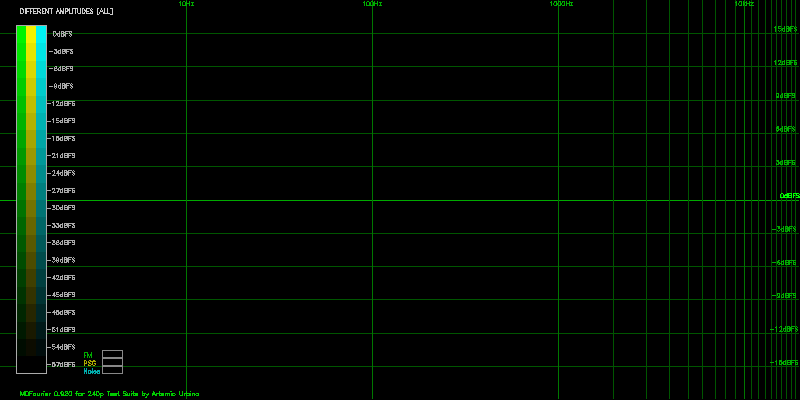
\includegraphics[width=1.0\linewidth]{images/interpretation/Plot1-SameFile.png}
	\caption[Same file compared]{Different Amplitudes result file when comparing the same file against itself}
	\label{fig:plot1-samefile}
\end{figure}

Of course all of the \textit{Differences} and \textit{Missing} plots will only have the grid and reference bars, with no plotted information since both input files are identical. 

However there will be two sets of \textit{Spectrograms}, one for the \textit{Reference} file and one for the \textit{Comparison} file, with one plot for each type plus the general one.

\begin{figure}[H]
	\centering
	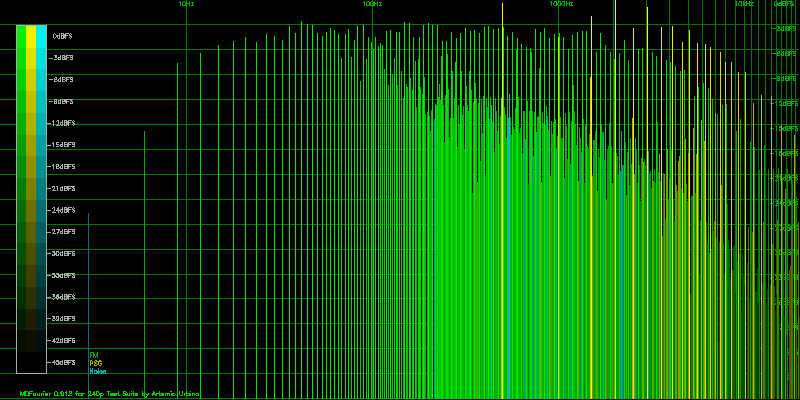
\includegraphics[width=1.0\linewidth]{images/interpretation/Plot2-SameFile-FM-Spectrogram.png}
	\caption[Spectrogram]{The Spectrogram for a Genesis 1 VA3 via hedphone out}
	\label{fig:plot2-samefile-fm-spectrogram}
\end{figure}

The Amplitude, or volume, of each of the fundamental \textit{sine waves} that compose the original signal is represented by vertical lines that reach from the bottom to the point that corresponds to the amplitude in \textit{dBFS} \cite{dbfs}. The line is also colored to represent that amplitude with the scale on the left showing the equivalence.

Three colors as defined from the \textit{mfn file}\footnote{The configuration file is described in appendix \ref{mfnconfig}} are used to plot the graph, with each one of them plotting the frequencies from each corresponding block from the \textit{WAV} file.

The top of the plot corresponds to the maximum possible amplitude, which is \textit{0 dBFS}. the bottom of the plot corresponds to the \textit{minimum significant volume}, as described in section \ref{MinSigVolume}.

Both sets of spectrograms in this case are identical, as expected. 

\section{Scenario 2: Comparing two different recordings from the same console}

This is another control case, what should we expect to see if we record two consecutive audio files from the same exact game console using the same sound card?

\begin{figure}[H]
	\centering
	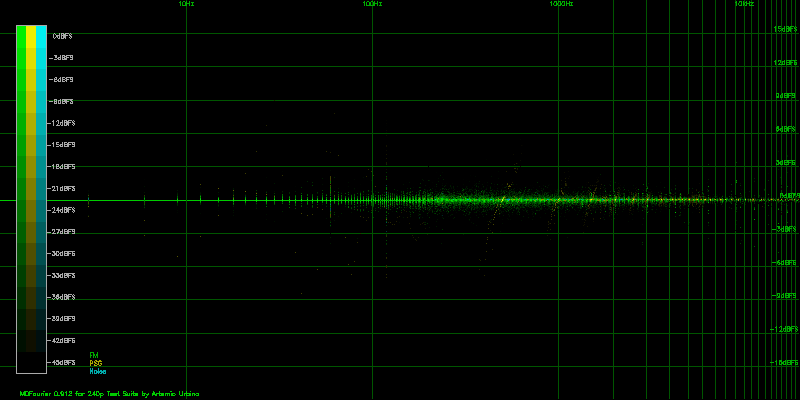
\includegraphics[width=1\linewidth]{images/interpretation/Plot2-Sameconsole.png}
	\caption[Same console compared]{The same console, two different recordings}
	\label{fig:plot2-sameconsole}
\end{figure}

As you can see, we have basically a flat line around zero. This means that there were no meaningful differences found. 

But wait, there \textit{are} differences. Why is that? Due to many reasons: analogue recordings are not always the same for one. Then we have variations from the analogue part of console itself, and probably from the internal states and clocks from the digital side. It can also be noise generated by differences in frequency bins when performing the \textit{DFT} after calculating the frame rates - we have that $\sfrac{1}{4}$ error after all.

We now know that there will be certain \textit{fuzziness}, or variation, around each plot due to this subtle recording and performance nuances. It is a normal situation that is to be expected, and a baseline for future results.

\section{Scenario 3: Comparing against a modified file}

For demonstration purposes, the same \textit{Reference} file was modified to add a \textit{500hz 6 dBFS} parametric equalization across all the analyzed signal. This is an artificially modified and controlled scenario in order to demonstrate what the plots mean.

\begin{figure}[H]
	\centering
	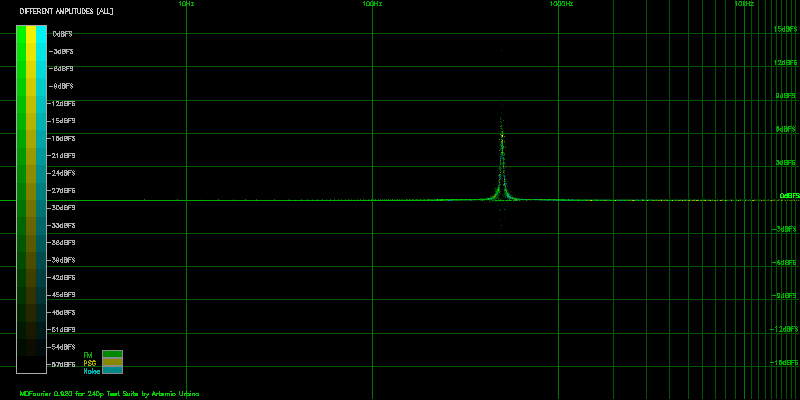
\includegraphics[width=1.0\linewidth]{images/interpretation/Plot3-Modified.png}
	\caption[1kHz modified]{Compared against itself modified with a \textit{500hz 6 db} equalization}
	\label{fig:plot3-modified}
\end{figure}

As expected all three blocks (\textit{FM}, \textit{PSG} and \textit{Noise}) were affected and show a spike, exactly \textit{6 dBFS} tall and centered around \textit{500hz}.

It is interesting to note both spectrograms, since the \textit{500hz} spike is also shown there.

\begin{figure}[H]
	\centering
	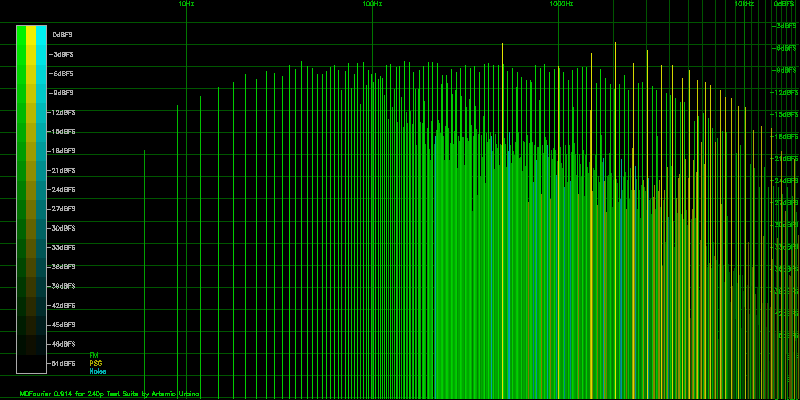
\includegraphics[width=1.0\linewidth]{images/interpretation/Plot3-Spectrogram.png}
	\caption[Reference File]{\textit{Reference} File}
	\label{fig:plot3-spectrogram}
\end{figure}

\begin{figure}[H]
	\centering
	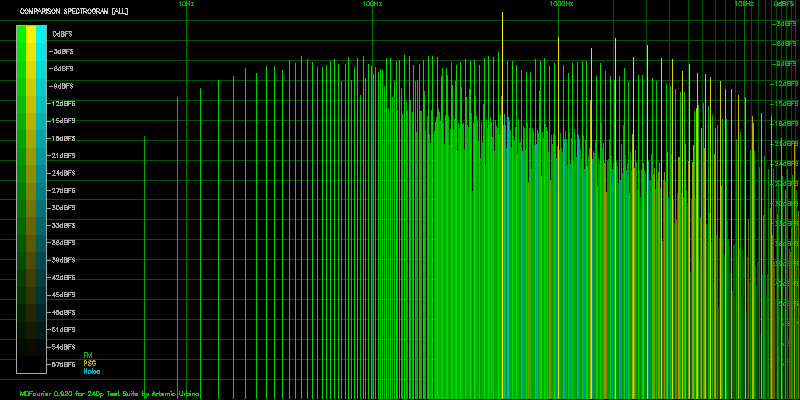
\includegraphics[width=1.0\linewidth]{images/interpretation/Plot3-Spectrogram-500hz.png}
	\caption[Reference File]{Reference file modified with \textit{500hz} peak}
	\label{fig:plot3-spectrogram-1kHz}
\end{figure}


And the \textit{Missing Frequencies} plots are basically empty, since no relevant frequencies are missing from the \textit{Comparison} file.

\section{Scenario 4: Comparing against digital low pass and high pass filters}

We'll use the same \textit{Reference} file, and compare it to a file with a several filters:

\begin{itemize}
	\item A \textit{low pass filter} to the \textit{FM} section of the file
	\item A steeper \textit{low pass filter} at a different cutoff frequency to the \textit{PSG} section
	\item A \textit{high pass filter} to the Noise section at a different frequency
\end{itemize}

This is the general plot with the three sections:

\begin{figure}[H]
	\centering
	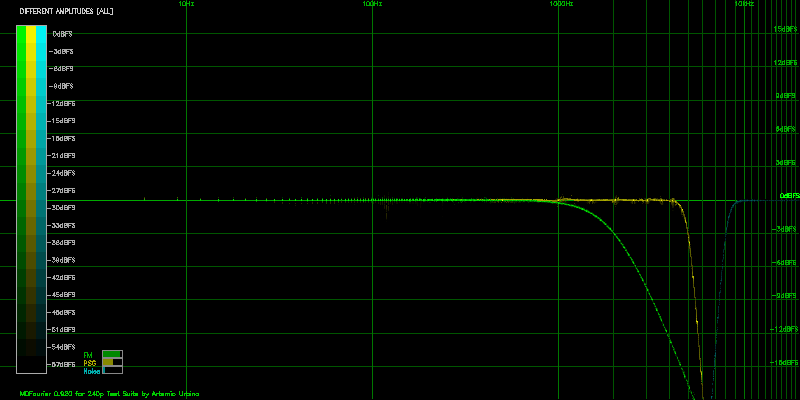
\includegraphics[width=1.0\linewidth]{images/interpretation/Plot4-1-All.png}
	\caption[All Plotted]{\textit{FM}, \textit{PSG} and \textit{Noise} with low pass, low pass and high pass filters}
	\label{fig:plot4-1-all}
\end{figure}

We can now see that the higher frequencies above \textit{1kHz} in the FM plot steeply go to \textit{$-\infty$ dBFS}, so the first low pass filter is there.

The second low pass filter for \textit{PSG} is at \textit{3kHz}, and is steeper.

But we can barely see what is going on with the \textit{Noise} part of the plot. We can see that there is some black dots on top of the \textit{0dBFS} line.

In order to better see what is going on, we'll change the \textit{color filter function} to $\sqrt{dbFS}$ so we can have higher contrast.\footnote{Described in section \ref{colorfilter})}

\begin{figure}[H]
	\centering
	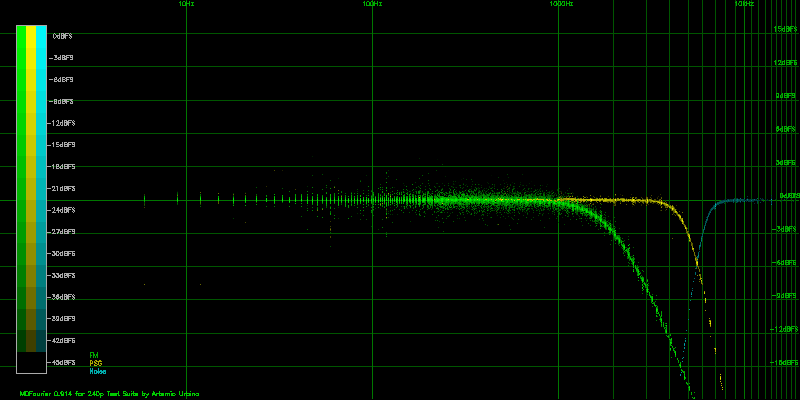
\includegraphics[width=1.0\linewidth]{images/interpretation/Plot4-2-All-sqrt.png}
	\caption[Using SQRT]{Using the $\sqrt{dbFS}$ color filter function}
	\label{fig:plot4-2-all-sqrt}
\end{figure}

With the higher contrast, we can now make out the curve that raises from \textit{$-\infty$ dBFS} to \textit{0 dBFS}, and it aligns with \textit{8kHz}.

We can still do a little bit better, by using the \textit{Average Plot} option.\footnote{An average and then a moving average are applied to the plot, see section \ref{usinggui} for details}

Here is the resulting plot for only the \textit{Noise} section of the signal with average enabled:

\begin{figure}[H]
	\centering
	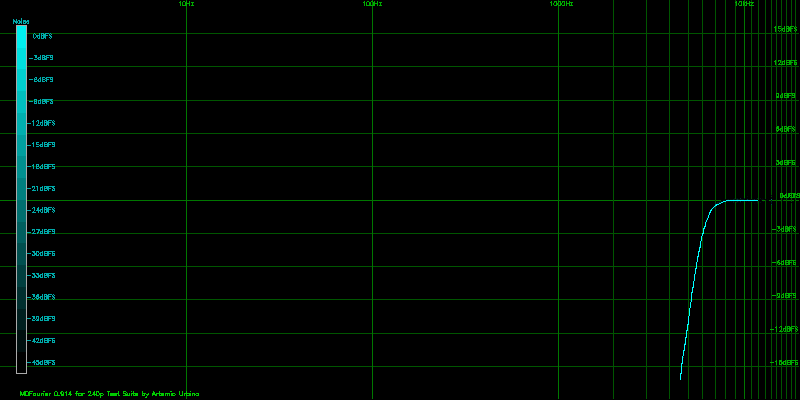
\includegraphics[width=1.0\linewidth]{images/interpretation/Plot4-3-AVG-Noise.png}
	\caption[Noise Average]{\textit{Noise} plot with Average}
	\label{fig:plot4-3-avg-noise}
\end{figure}

There are some other interesting plots that result from this experiment. For example, the \textit{Missing} plots now show all the frequencies the \textit{low/high pass} filters cut off.

\begin{figure}[H]
	\centering
	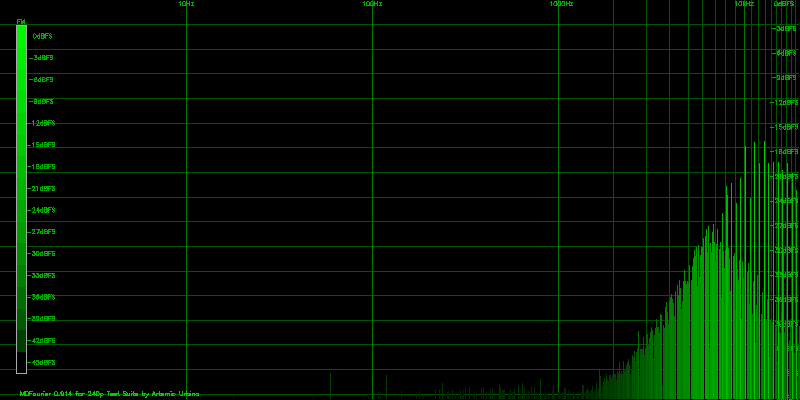
\includegraphics[width=1.0\linewidth]{images/interpretation/Plot4-4-Missing-FM.png}
	\caption[Missing FM]{Missing frequencies in \textit{FM} cutoff by low pass filter}
	\label{fig:plot4-4-missing-fm}
\end{figure}

As show in figure \ref{fig:plot4-4-missing-fm}, there is a curve in the spectrogram and only frequencies above \textit{1kHz} show up, slowly rising in amplitude.

\begin{figure}[H]
	\centering
	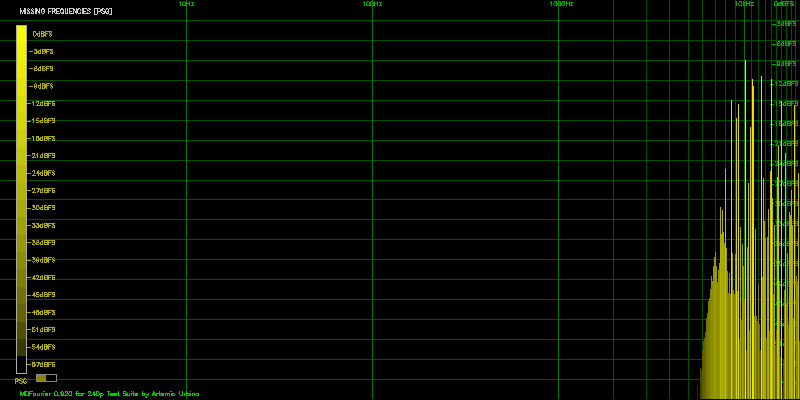
\includegraphics[width=1.0\linewidth]{images/interpretation/Plot4-5-Missing-PSG.png}
	\caption[Missing PSG]{Missing frequencies in \textit{PSG} cutoff by low pass filter}
	\label{fig:plot4-5-missing-psg}
\end{figure}

The same behavior can be observed in the \textit{PSG spectrogram}, but with a different curve that starts at \textit{4kHz} in figure \ref{fig:plot4-5-missing-psg}.

\begin{figure}[H]
	\centering
	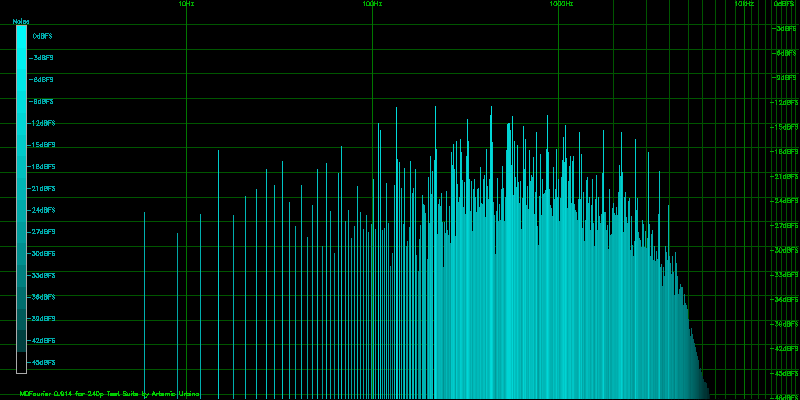
\includegraphics[width=1.0\linewidth]{images/interpretation/Plot4-6-Missing-Noise.png}
	\caption[Missing Noise]{Missing frequencies in \textit{Noise} cutoff by high pass filter}
	\label{fig:plot4-6-missing-noise}
\end{figure}

And finally, figure \ref{fig:plot4-6-missing-noise} shows the opposite kind of curve, the \textit{high pass filter} cuts off everything higher than \textit{8kHz} in the \textit{Noise} section.

It is a good moment to emphasize that these are relative plots. They show how different the \textit{Comparison} signal is to the \textit{Reference} signal. And so far we've compared the same signal to itself although modified with very precise digital manipulations. An analog filter would look the same, but a bit fuzzier. 

However, some interesting ideas arise. What would happen if we take this \textit{low/high pass filte}r signal and use it as \textit{Reference} and the original one as \textit{Comparison}?

\begin{figure}[H]
	\centering
	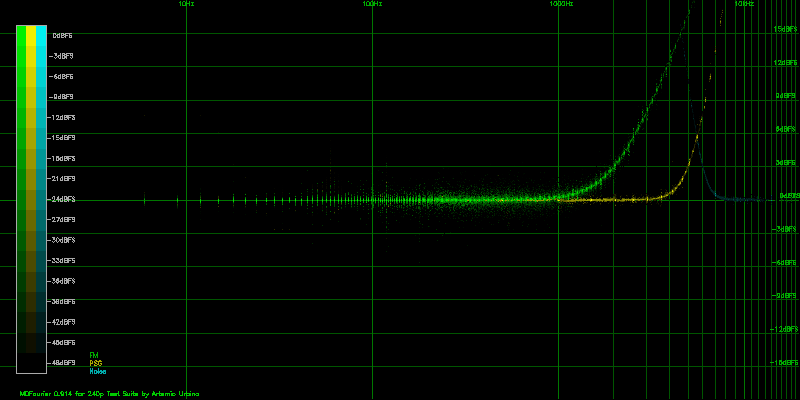
\includegraphics[width=1.0\linewidth]{images/interpretation/Plot4-7-Reversed.png}
	\caption[Reversed]{Results when using modified signal as \textit{Reference}}
	\label{fig:plot4-7-reversed}
\end{figure}

Based on this, one could jump to the conclusion that everything will simply be inverted. After all, the original signal now rises to \textit{$+\infty$ dBFS} at the same spots - and that makes complete sense -  since those frequencies now have a higher amplitude. 

Although the \textit{Differences} and \textit{Spectrogram} plots will indeed be inverted under these controlled conditions, the \textit{Missing} plots are different. Most of them are now empty:

\begin{figure}[H]
	\centering
	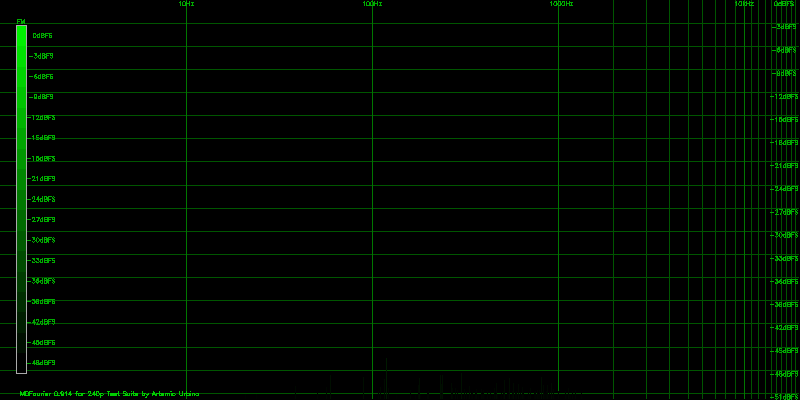
\includegraphics[width=1.0\linewidth]{images/interpretation/Plot4-8-Missing-FM-Inverted.png}
	\caption[Reversed FM Missing]{\textit{Missing Frequencies} plot for \textit{FM} is empty}
	\label{fig:plot4-8-missing-fm-inverted}
\end{figure}

This happens because we cut a lot of frequencies with such steep \textit{low} and \textit{high pass filters}, and all the frequency content from this modified signal is present in the original, but not the other way around as we saw before.

\section{Scenario 5: Comparing two recordings from the same console made with different Audio Cards}

We'll now compare the same console using two different recordings, one made with an internal \textit{PCI M-Audio 192} and the other with a \textit{USB Lexicon Alpha}. Here are the results:

\begin{figure}[H]
	\centering
	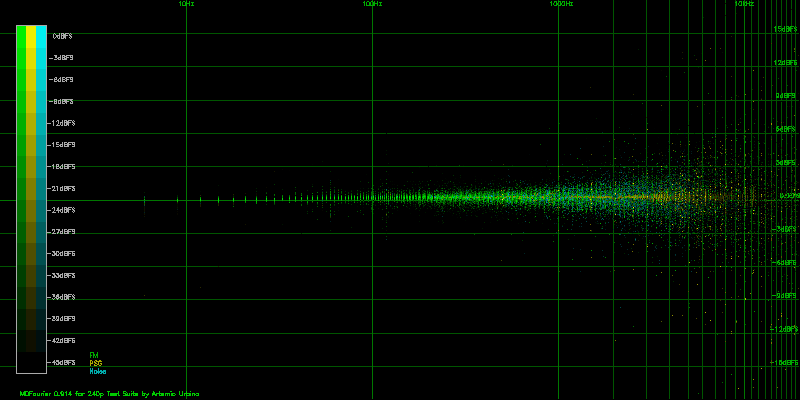
\includegraphics[width=1.0\linewidth]{images/interpretation/Plot5-1-All.png}
	\caption[Reversed FM Missing]{Differences using same hardware and cables, different capture cards}
	\label{fig:plot5-1-all}
\end{figure}

Well, I am guessing that was unexpected. We can tell a few things though. First, the frequency response is slightly different, since we now have that \textit{scatter} at the higher end of the spectrum, in what is commonly referred as \textit{treble}.

But we can still clearly tell that the scatter is centered around the \textit{0 dBFS} line, which means that even using different sound cards we can tell the differences between systems\footnote{Under the assumption both cards have a relatively flat frequency response, like the ones used here. See the Audio Cards appendix for specifications \ref{audiocards}}. 

Also, there was a slight difference in the detected frame rates. This happens since the sampling clock in not exactly the same in both audio cards. Here is the output text from the analysis that shows the detected frame rates:

\begin{verbatim}
* Loading 'Reference' audio file A-MD1UTVA3_M-192.wav
- WAV file is PCM 44100hz 16bits and 63.51 seconds long
- Starting sync pulse train:  1.25499s [221380 bytes]
- Trailing sync pulse train:  59.0045s [10408396 bytes]
- Detected 59.914 hz video signal (16.6906ms per frame) from WAV file

* Loading 'Comparison' audio file A-MD1UTVA3-lexicon.wav
- WAV file is PCM 44100hz 16bits and 60.39 seconds long
- Starting sync pulse train:  1.30923s [230948 bytes]
- Trailing sync pulse train:  59.0523s [10416824 bytes]
- Detected 59.9208 hz video signal (16.6887ms per frame) from WAV file
\end{verbatim}

The \textit{USB Lexicon alpha} has a more accurate sampling clock, although the difference is minimal\footnote{We are talking 0.0019ms in this case, that is 0.0000019 seconds!} and \textit{MDFourier} compensates for such issues.\footnote{The expected frame rate from the vintage console analyzed here is \textit{16.688ms} per frame, or 59.92hz as measured with a scope. See appendix \ref{framerate}}

Here is the graph with the \textit{Average plot} option turned on.

\section{Scenario 6: Comparing wav vs mp3}
\label{mp3}

\section{Scenario 7: Comparing two vintage consoles}

\section{Corner cases}
\label{cornercase}

\chapter{Results from vintage retail hardware}

The following table lists all the hardware used to make the recordings for the following result plots for this chapter. All systems had stock parts at the time of recording, no modifications and used original power supplies. 

They were all connected to a 4" \textit{CRT} via \textit{RGB}, although the \textit{CRT} was turned off while recording\footnote{Video Refresh noise is indeed detected by the software, but since it is such an isolated frequency range - at a sharp 20 hz - it is not filtered out for comparisons.}.

For simplicity, the recordings shown were made using the \textit{USB Lexicon Alpha} audio card\footnote{See appendix \ref{audiocards}}. All the recordings are available from the \textit{downloads page} from the \textit{MDFourier} website\footnote{URL is \url{http://junkerhq.net/MDFourier/}}.

The \textit{MDFourier ID} value in the following table refers to the name of the files in the catalogue.

\begin{center}
\scalebox{0.6}{
\begin{tabular}{ | l | l | l | l | l | l | l | l | l | }
    \hline
	Type    & Model    & Revision & FCCID & Serial & Region & Made in & MDFourier ID & Recorded from\\
    \hline
	Model 1 & HAA-2510 & VA1    &               & 89N61751  & Japan & Japan  & A-MD1JJVA1   & Headphone Out\\
	Model 1 & 1601     & VA3    & FJ846EUSASEGA & 30W59853  & USA   & Taiwan & A-MD1UTVA3   & Headphone Out\\
	Model 1 & 1601     & VA6    & FJ8USASEGA    & B10120356 & USA   & Japan  & A-MD1UJVA6   & Headphone Out\\
	Model 1 & 1601     & VA6    & FJ8USASEGA    & 59006160  & USA	& Taiwan & A-MD1UTVA6-1 & Headphone Out\\
	Model 1 & 1601     & VA6    & FJ8USASEGA    & 31X73999  & USA   & Taiwan & A-MD1UTVA6-2 & Headphone Out\\
	Model 1 & HAA-2510 & VA6    &               & A10416197 & Japan	& Japan  & A-MD1JJVA6   & Headphone Out\\
	Model 2 & MK-1631  & VA1.8  & FJ8MD2SEGA    & 151014280 & USA   & China  & A-MD2UCVA18  & AV Out\\
	Nomad   & MK-6100  &        & 50059282	    &           & USA	& Taiwan & A-NMUT       & Headphone Out\\
	CDX     & MK-4121  &        & Y40 014198    &           & USA   & Japan  & A-CDXUJ-LO   & Line Out\\
	CDX     & MK-4121  &        & Y40 014198    &           & USA   & Japan  & A-CDXUJ-HP   & Headphone Out\\
	\hline
\end{tabular}
}
\end{center}

\section{Sega Genesis Model 1 VA3 (US) vs Mega Drive Model 1 VA1 (JP)}

\section{Sega Genesis Model 1 VA3 (US) vs Sega Genesis Model 1 VA6 (JP)}

\section{Sega Genesis Model 1 VA6 (US) vs Mega Drive Model 1 VA6 (JP)}

\section{Sega Genesis Model 1 VA6 (US) vs Sega Genesis Model 1 VA6 (US)}

\section{Sega Genesis Model 1 VA3 (US) vs Sega Genesis Model 2 VA1.8 (US)}

\section{Sega Genesis Model 1 VA3 (US) vs Sega CDX (US)}

\section{Sega Genesis Model 1 VA3 (US) vs Sega Nomad (US)}

\section{Sega CDX (US) Line-out vs Sega CDX (US) Headphone port}

\begin{appendices}
	
\chapter{Licensing}

\textit{MDFourier} Copyright (C)2019 Artemio Urbina
\label{license}
This program is free software: you can redistribute it and/or modify
it under the terms of the GNU General Public License as published by
the Free Software Foundation, either version 3 of the License, or
(at your option) any later version.

This program is distributed in the hope that it will be useful,
but WITHOUT ANY WARRANTY; without even the implied warranty of
MERCHANTABILITY or FITNESS FOR A PARTICULAR PURPOSE.  See the
GNU General Public License for more details.

You should have received a copy of the GNU General Public License
along with this program.  If not, see \url{https://www.gnu.org/licenses/}.	
	
\chapter{Configuration file}
\label{mfnconfig}

All these parameters are defined in the file \textit{mdfblocks.mfn}\footnote{This is the default file name, a different file can be used and selected via the command line. In future \textit{Front End} revisions it might be selected via a combo box. One for each supported hardware profile}. Here is the current file we are using to compare \textit{Mega Drive/Genesis} audio characteristics:

\begin{verbatim}
MDFourierAudioBlockFile 1.0
MegaDriveAudio
16.688
8820 -25 25 14 18 10
7
Sync s 1 20 red
Silence n 1 20 red
FM 1 96 20 green
PSG 2 60 20 yellow
Noise 3 14 20 aqua
Silence n 1 20 red
Sync s 1 20 red
\end{verbatim}

This file defines what \textit{MDFourier} must do and how to interpret the WAV files. For now it can read \textit{44kHz} and \textit{48kHz} files, in \textit{Stereo PCM} format\footnote{This is more than enough for the human hearing spectrum \cite{MontyMontgomery}}.

The first line is just a header, so that the program knows it is a valid file and in the current format.

The second line is the name of the current configuration, since I plan to add support for any console or arcade hardware in the future. This would imply creating a new \textit{mfn} file for each configuration, and a specific binary to be run on the hardware.

The third line is the expected frame rate. This is only used as a reference to estimate the placement for the blocks within the file before calculating the frame rate as captured by the audio capture card. After that is calculated, each file uses its own definition in order to be fully aligned. Variations in the detected frame rate are natural, since we have an error of $\sfrac{1}{4}$ of a millisecond\footnote{For reference $\sfrac{1}{4}$ of a millisecond corresponds to 0.00025 seconds. Modern systems have different frame rates adapted for modern displays, small differences are more likely caused by the audio capture hardware \cite{SoundCardClock}}, dictated by the sample rates and audio card limitations.

The fourth line defines the characteristics of the pulse tone used to identify the starting and end points of the signal within the wave file. Its frequency, relative \textit{amplitude difference} to the \textit{background noise} (silence), and length \textit{intervals} that will be better explained in future revisions of this document.

The fifth line defines how many different blocks are to be identified within the files. There are seven blocks in this case.

Each block is composed of five characteristics: A \textit{Name}, a \textit{type}, the \textit{total number of elements} that compose it, each element \textit{duration} specified in frames and the \textit{color}\footnote{Available colors are listed in Appendix \ref{availablecolors}} to be used for identifying it when plotting the results. Each block must correspond to a line with these parameters.

For example, FM audio has been named \textit{"FM"}, type \textit{1}, \textit{96} elements of \textit{20} frames each and will be colored in \textit{green}. Definition is in frames since emulators and \textit{FPGA} implementations tend to run at different frame rates than the vintage retail platform, which result in different durations. The only way to align them, is by respecting the driving force that tied this up in the old days: the video signal.

There are currently two special types, identified by the letters \textit{'s'} and \textit{'n'}. The first one defines a \textit{sync pulse}, which is used to automatically recognize the starting and ending points of the signal within the wave file. 

The second one is for null audio, or silence. This \textit{silence} is used to measure the \textit{background noise}\footnote{How analysis is affected by this is described in section \ref{MinSigVolume}} as recorded by the audio card. 	
	
\chapter{MDWave}
\label{mdwave}

\textit{MDWave} is a companion command line tool to \textit{MDFourier}. During development and while learning about \textit{DSP}, I needed to check what I was doing in a more tangible way. So in order to visualize the files in an audio editor and listen to the results \textit{MDWave} was born.

It takes a single wave file as argument, and loads all the parameters defined in the configuration file in order to verify the same environment. (see section \ref{mfnconfig}).

The output is stored under the folder \textit{MDWave}, and a subfolder with the name of the input \textit{WAV} file. The default output is a \textit{Wave} file named \textit{Used} which has the reconstructed signal from the original file after removing all frequencies that were discarded by the parameters used.

This means that it does a \textit{Fourier Transform}, applies the selected \textit{window} (section \ref{windows}) and estimates the noise floor. The highest amplitude frequencies are identifies and limited by range for each element defined in the configuration file, and rest are discarded. An \textit{Inverse Fourier Transform} is applied in order to reconstruct the wave file and the results are saved.

The opposite can be done as well by specifying the \textit{-x} option, and the result is a \textit{Discarded} wave file, that has all the audio information that was deemed irrelevant and discarded by the specified options. With this you can listen to these and determine if a more severe comparison is needed.

In addition, the \textit{-c} option creates a wave file with the chunk that corresponds to each element from the \textit{Reference} file being used, trimmed using the detected frame rate. Two chunks are created for each element, the \textit{Source} wav chunk has the element trimmed without modification and the \textit{Processed} wav chunk has the same element but with the windows and frequency trimming applied.

It has a few more command line options, which I'll detail in later versions of the document. You can type \textit{mdwave -h} in your \textit{mdfourier} folder for details.

\chapter{Window Function equations and plots}
\label{windowfunctiondetails}

This appendix lists the equation and curve of each \textit{Window Function} used to limit \textit{spectral leakage} as described in section \ref{windows}.

\newpage
\section{Tukey}

The default is a \textit{Tukey} window selected for this purpose. It uses $\alpha = 0.6$, zeroing just a few samples, with minimal \textit{spectral leakage} and good amplitude response.

The following equation is used to create the slopes:

\begin{equation}
tukey(x)=\frac{1}{2}(1+\cos(\frac{\pi(|x-\frac{N-1}{2}|-\alpha \frac{N-1}{2})}{(1-\alpha)\frac{N-1}{2}}))
\end{equation}

And this is the resulting plot of the \textit{Tukey} window, ranges are 0.0 to 1.0 horizontally and -0.1 to 1.1 vertically.

\begin{figure}[H]
	\centering
	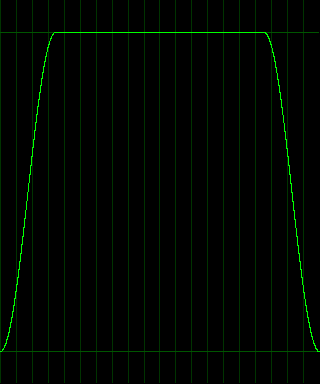
\includegraphics[width=0.4\linewidth]{images/windows/window-tukey.png}
	\caption[Tukey Window]{Tukey window used by \textit{MDFourier}, vertical lines are frames on a 20 frame signal}
	\label{fig:window-tukey}
\end{figure}

Detailed information can be found in the reference webpage \cite{tukey}.

\newpage
\section{Hann}
When selected, a typical \textit{Hann} window is used. This should be used to get the last \textit{spectral leakage}, with a very small trade off in amplitude accuracy.

\begin{equation}
hann[x] = \frac{1}{2}(1 - \cos(\frac{2\pi(x+1)}{n+1}))
\end{equation}

\begin{figure}[H]
	\centering
	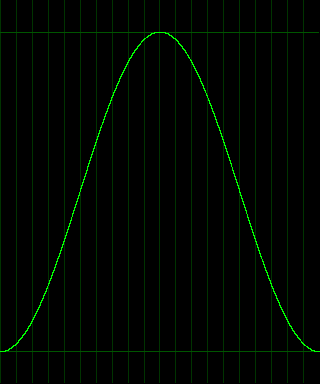
\includegraphics[width=0.4\linewidth]{images/windows/window-hann.png}
	\caption[Hann Window]{Hann Window}
	\label{fig:window-hann}
\end{figure}

\newpage
\section{Flattop}
A typical \textit{Flat top} window is used, selecting this will target amplitude accuracy against frequency bin precision.

\begin{align*}
flattop(x)=0.21557895 - 0.41663158\cos(2\pi\frac{x}{n-1})+ 0.277263158\cos(4\pi\frac{x}{n-1})\\
- 0.083578947\cos(6\pi\frac{x}{n-1}) + 0.006947368\cos(8\pi\frac{x}{n-1})
\end{align*}

\begin{figure}[H]
	\centering
	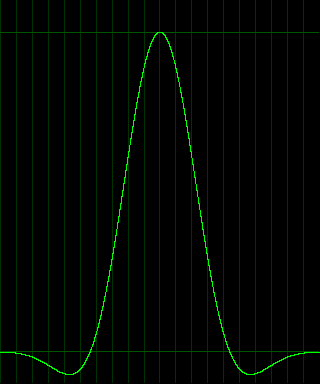
\includegraphics[width=0.4\linewidth]{images/windows/window-flattop.png}
	\caption[Flat Top window]{Flat Top window}
	\label{fig:window-flattop}
\end{figure}

\newpage
\section{Hamming}
A typical \textit{Hamming} window is used, presented for completeness and reference since the samples are never zeroed out.

\begin{equation}
hamming[x] = 0.54 - 0.46\cos(\frac{2\pi x}{n-1})
\end{equation}

\begin{figure}[H]
	\centering
	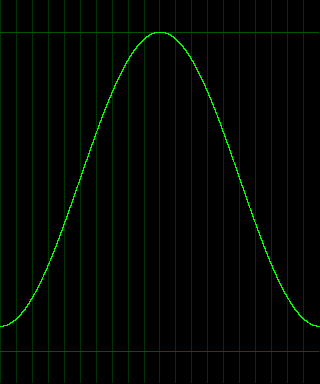
\includegraphics[width=0.4\linewidth]{images/windows/window-hamming.png}
	\caption[Hamming window]{Hamming window}
	\label{fig:window-hamming}
\end{figure}


\section{No Window}

No window is applied to the signal before applying the \textit{DFT}, equivalent to a \textit{rectangular window}. This leaves the signal unprocessed and any uncontrolled decay and audio card noise will be factored in as part of the periodic signal.

There is more information on windows and their usage in the reference webpage \cite{windowtypes}.

\chapter{Color Filter Function details}
\label{filterfunctions}

This appendix contains a description, plot and example of each \textit{Color Filter Function} from section \ref{colorfilter}.

\newpage
\section{None} 

No filtering is applied, as a result all differences are plotted with the brightest color. 

\begin{figure}[H]
	\centering
	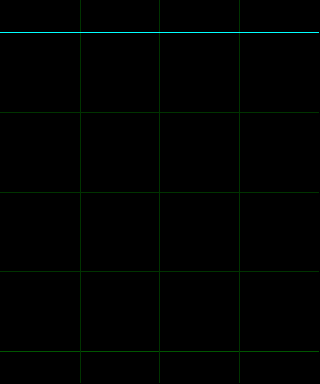
\includegraphics[width=0.4\linewidth]{images/colorfilter/BetaFunctionPlot_0.png}
	\caption[No Filter]{No Filter}
	\label{fig:betafunctionplot0}
\end{figure}

\begin{figure}[H]
	\centering
	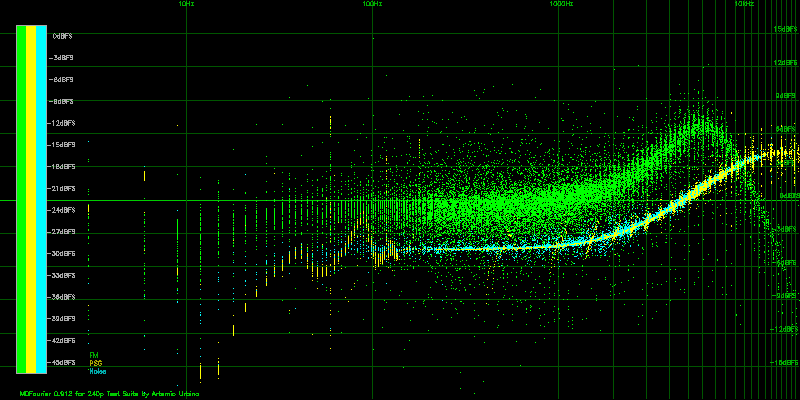
\includegraphics[width=1\linewidth]{images/colorfilter/BetaFunctionPlot_0_Data.png}
	\caption[No Filter]{No Filter Applied}
	\label{fig:betafunctionplot0data}
\end{figure}

\newpage
\section{$\sqrt{dbFS}$} 

A square root function will only attenuate the lowest amplitude differences.

\begin{figure}[H]
	\centering
	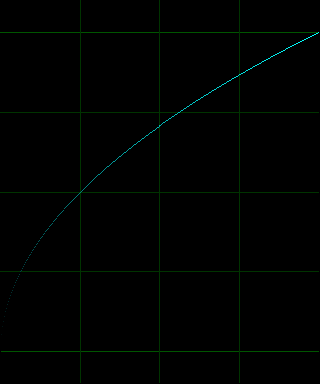
\includegraphics[width=0.4\linewidth]{images/colorfilter/BetaFunctionPlot_1.png}
	\caption[Square Root filter]{Square Root filter}
	\label{fig:betafunctionplot1}
\end{figure}

\begin{figure}[H]
	\centering
	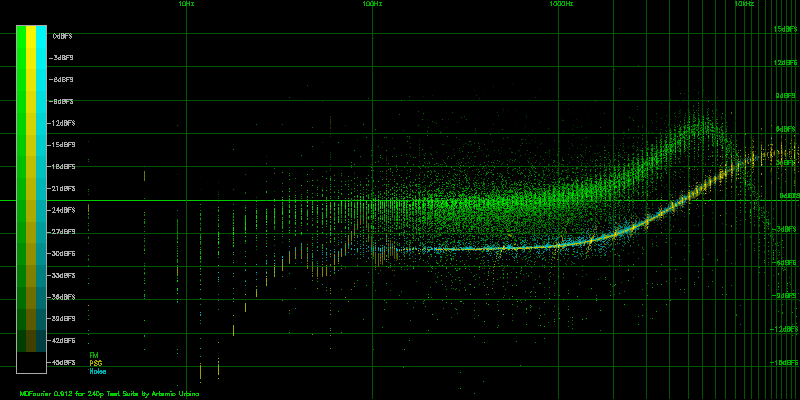
\includegraphics[width=1\linewidth]{images/colorfilter/BetaFunctionPlot_1_Data.png}
	\caption[Square Root filter]{Square Root filter Applied}
	\label{fig:betafunctionplot1data}
\end{figure}

\newpage
\section{$\beta(3,3)$}

A Beta Function filter with parameters (3, 3) will attenuate a bit more from the lower range, still showing most of the differences.

\begin{figure}[H]
	\centering
	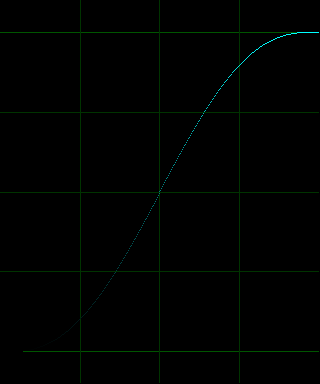
\includegraphics[width=0.4\linewidth]{images/colorfilter/BetaFunctionPlot_2.png}
	\caption[Beta Function(3,3)]{Beta Function(3,3)}
	\label{fig:betafunctionplot2}
\end{figure}

\begin{figure}[H]
	\centering
	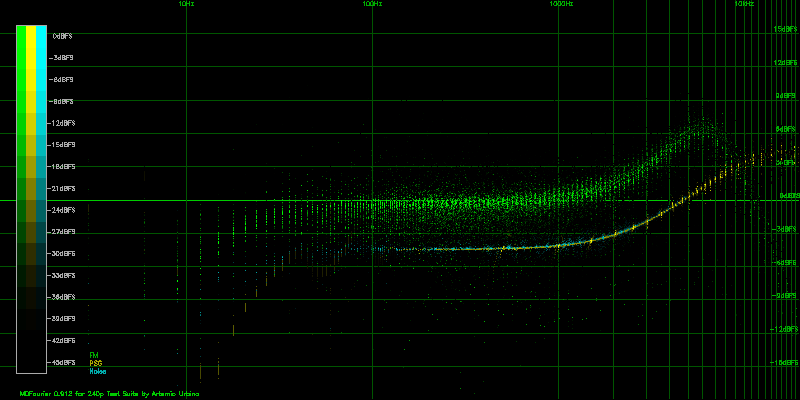
\includegraphics[width=1\linewidth]{images/colorfilter/BetaFunctionPlot_2_Data.png}
	\caption[Beta Function(3,3)]{Beta Function(3,3) Applied}
	\label{fig:betafunctionplot2data}
\end{figure}

\newpage
\section{$Linear$} 

The linear function is the default, and has no bias. Half the dinamic range corresponds to half the color rage.

\begin{figure}[H]
	\centering
	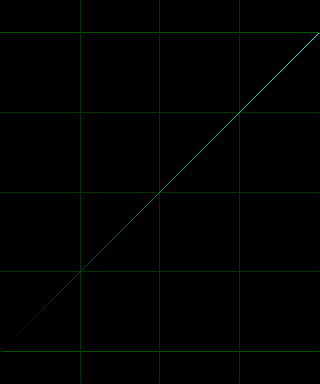
\includegraphics[width=0.4\linewidth]{images/colorfilter/BetaFunctionPlot_3.png}
	\caption[Linear]{Linear Function}
	\label{fig:betafunctionplot3}
\end{figure}

\begin{figure}[H]
	\centering
	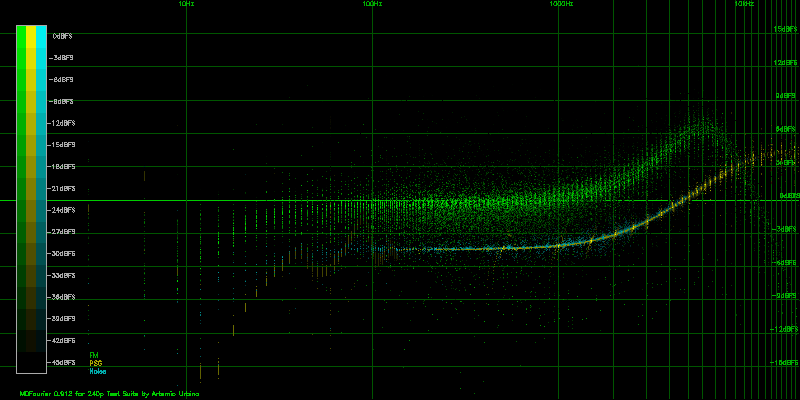
\includegraphics[width=1\linewidth]{images/colorfilter/BetaFunctionPlot_3_Data.png}
	\caption[Linear Applied]{Linear Function Applied}
	\label{fig:betafunctionplot3data}
\end{figure}

\newpage
\section{$dBFS^2$}

A squared function will attenuate a lot more differences, as a result frequencies with the highest amplitude in the reference signal will be brighter.

\begin{figure}[H]
	\centering
	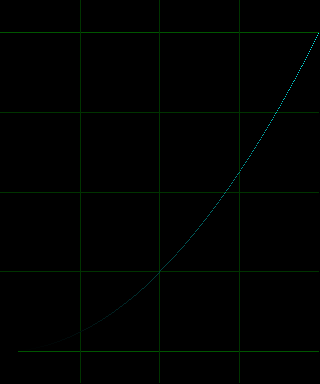
\includegraphics[width=0.4\linewidth]{images/colorfilter/BetaFunctionPlot_4.png}
	\caption[Linear]{Linear Function}
	\label{fig:betafunctionplot4}
\end{figure}

\begin{figure}[H]
	\centering
	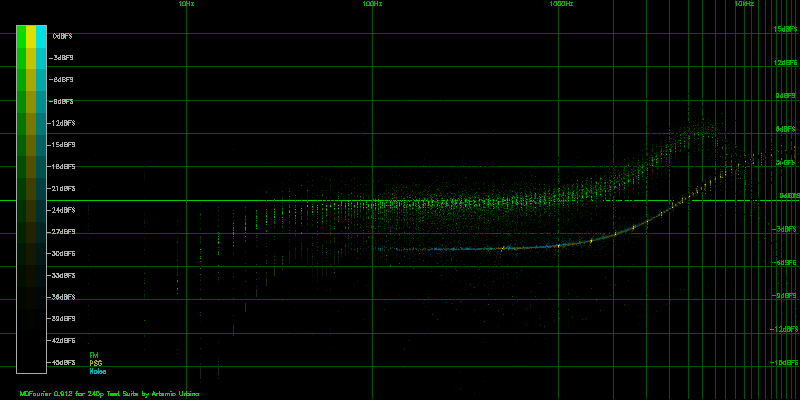
\includegraphics[width=1\linewidth]{images/colorfilter/BetaFunctionPlot_4_Data.png}
	\caption[Linear Applied]{Linear Function Applied}
	\label{fig:betafunctionplot4data}
\end{figure}

\newpage
\section{$\beta(16,2)$} 

A Beta Function filter with parameters (16,2) will attenuate almost all the differences, and only the frequencies with the highest amplitude in the reference signal will be brighter.

\begin{figure}[H]
	\centering
	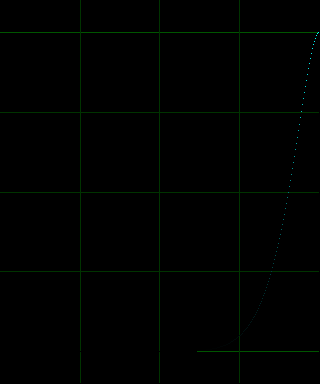
\includegraphics[width=0.4\linewidth]{images/colorfilter/BetaFunctionPlot_5.png}
	\caption[Beta Function(16,2)]{Beta Function(16,2)}
	\label{fig:betafunctionplot5}
\end{figure}

\begin{figure}[H]
	\centering
	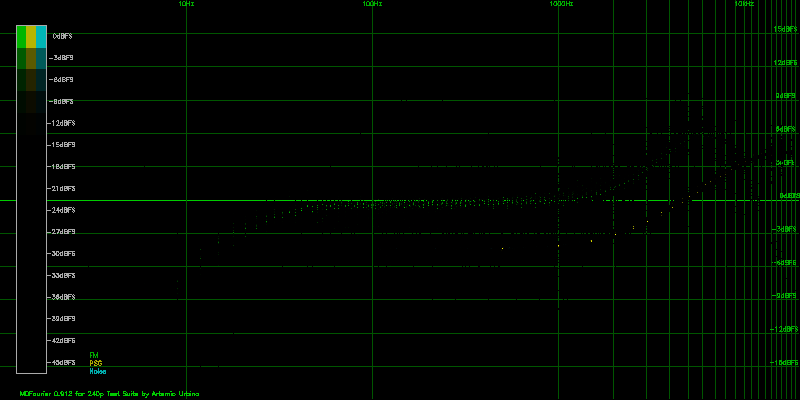
\includegraphics[width=1\linewidth]{images/colorfilter/BetaFunctionPlot_5_Data.png}
	\caption[Beta Function(16,2)]{Beta Function(16,2) Applied}
	\label{fig:betafunctionplot5data}
\end{figure}

\chapter{Normalization and amplitude matching}
\label{normalization}

Since each signal is probably at its own distinct volume, we need to perform a a \textit{normalization} process in order to have a common compare point between them.

Each type of \textit{normalization} has its own strengths and weaknesses, but the \textit{frequency domain} normalization designed for this process is always accurate with respect o the \textit{Reference} signal, but might be confusing in some corner cases\footnote{One such example is available in section \ref{cornercase}} if the underlying causes are not well understood when interpreting the results.

Since silence can't be used as reference\footnote{Noise floor will vary by console and by audio card}, the only other option is fixing points from within the signal. Every normalization process used follows a different logic for fixing one such point for comparison.

The default is to do this in the \textit{frequency domain}\footnote{This means it is performed after the Discrete Fourier Transform and using the data generated by it.}, but there are two other options available via command line\footnote{These can be enabled via the \textit{extra command} option from the GUI as explained in section \ref{extracommand}}. All three methods are described in the following sections.

\section{Frequency domain normalization}

This is the default option used my the software. It involves finding the \textit{highest magnitude}\footnote{At this point in the analysis there are no amplitudes defined, since we have no reference points. Hence we don't use amplitude, and raw magnitude values from each transform are used.} from the \textit{Fourier Transform} of the \textit{Reference} signal before amplitudes are calculated. Then a corresponding match in the \textit{Comparison} signal's frequency spectrum for the same block is searched for. 

This means that the exact same fundamental frequency with the highest magnitude value is searched for, occurring at the same position in time - which corresponds to the block. Having both points, a meaningful \textit{reference point} is set for the comparison, and the relative amplitudes between the signals can be calculated.

In order to calculate the amplitudes, \textit{0dBFS} is matched against the absolute highest magnitude from the \textit{Comparison} file\footnote{Since the highest point of the \textit{Reference} signal was matched to one other point in the \textit{Comparison} file, there are only two options: either both peaks are in the exact same spot, or there is a higher peak in the \textit{Comparison} file}, after both signals have been relatively normalized in amplitude against the reference point.

This method has shown to be always accurate within the tests. However, results can be unexpected in certain corner cases as the one shown in section \ref{cornercase}. 

\section{Time domain normalization}

The process is very similar to the \textit{frequency domain} variant but it is done using the raw audio samples directly from the \textit{WAV} file\footnote{Values are changed only in RAM during execution, input files are never modified}.

The highest amplitude is searched for within the samples of the meaningful audio signal, as dictated by the configuration file\footnote{Described in section \ref{mfnconfig}}. The corresponding segment in time is then located in the \textit{Comparison} file, and a pre-defined duration\footnote{One frame in the current implementation} is searched for the sample with the \textit{maximum local} value.

The \textit{Comparison} signal is then absolutely normalized to \textit{0dBFS}\footnote{Relative to \textit{0xFFFF} - the top value in \textit{16 bit} samples in the \textit{WAV} file}, and the \textit{Reference} signal is then relatively normalized using the adjusted \textit{local maximum} value. This follows the same rationale described for the \textit{frequency domain} equivalent.

Although the results can sometimes be deceivingly familiar, they are not correctly referenced in corner cases\footnote{See section \ref{cornercase} for an example}, and they do not represent the real relation between the signals. However, they can be useful for analysis while in the process of understanding how to interpret the plots.

\section{Highest fundamental average normalization}

This normalization option also takes place in the \textit{frequency domain}. The idea is to average the highest magnitudes - the fundamentals - from all segments and use the resulting ratio calculated between both signals to normalize them.

The results are always centered around the \textit{0dBFS} line in the \textit{Differences plot}, allowing a globalized view. However, the amplitude differences are not to be relied upon for calibration, since they are not relative to a fixed point from the \textit{Reference} signal. This option is just available for cases when both signals present a high difference rate between them, which is unexpected but possible.

\chapter{Frame rates and their importance}
\label{framerate}

The \textit{frame rate} is the amount of frames per second a system sends to the display. Since the \textit{custom binary} runs from within the target system, we are subject to the internal timing. Every time a frame starts the process for being sent to the display, an event called \textit{vertical sync} occurs. This is the driving clock for the whole console\footnote{As a matter of fact, almost all the code for running games - or the custom binary in out case - is executed during a segment called \textit{vertical blank}.}.

It is vital for the process to have a basic unit of time, in order to segment the file in the chunks needed for analysis and to send the correct values to the \textit{Discrete Fourier Transform}.

Signals generated from different sources can have dissimilar \textit{frame rates}, even when running the same programs and representing the same platform. This can be due to several reasons: having a different display technology as target, hardware inconsistencies between revisions, etc.

Another source for variation is the audio capture device, since these can vary slightly in their sample rate clocks. But usually these are lower variations that are reported and compensated for internally.

The frame duration is the basic unit of measurement, since we are dealing with signals that are well below one second. Because of this, the configuration file\footnote{See appendix \ref{mfnconfig}} defines the expected frame duration in milliseconds as measured from a vintage console. One such example is the frame duration as measured from an \define{ntsc} \textit{Sega Genesis} using an \textit{oscilloscope}\footnote{Electronic tool for measuring electric signals.} as shown in figure \ref{fig:frameratescope}.

\begin{figure}[H]
	\centering
	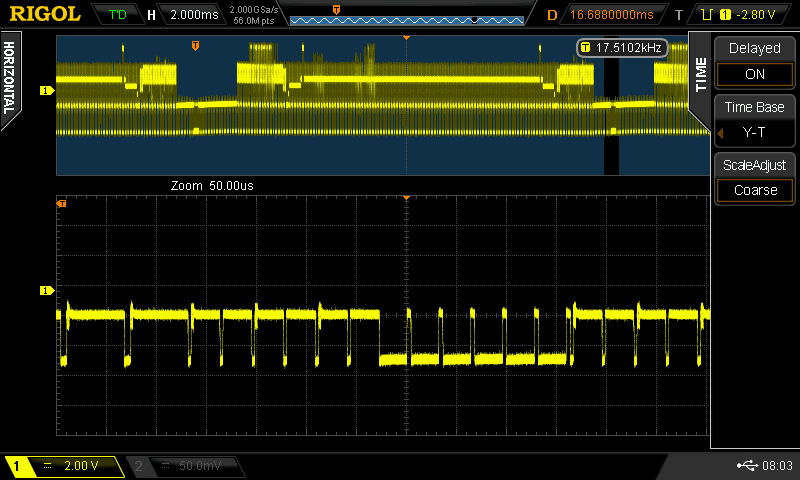
\includegraphics[width=1.0\linewidth]{images/scope/framerate-scope.png}
	\caption[Scope frame rate]{Frame duration as measured with a scope from a \textit{Model 1 VA3 system}}
	\label{fig:frameratescope}
\end{figure}

The oscilloscope shows a frame duration of \textit{16.888ms}, and this is the value used in the configuration file\footnote{Described in appendix \ref{mfnconfig}} for the initial frame rate calculations.

After the \textit{sync pulses} are detected\footnote{Described in appendix \ref{mfnconfig}}, a new frame rate value is calculated from the audio file. This new frame rate is used across the whole process, and can vary from the vintage console due to a combination of different reasons.

Every audio card can have a slightly different \textit{sample clock}\footnote{See appendix \ref{audiocards}}, and this variation will affect the starting and ending points within the recording. Such variation can be detected and estimated from the audio signal, and it is reported if the \textit{verbose log}\footnote{See section \ref{verbose}} option is enabled.

The selected \textit{sample rate} for recording can also affect the \textit{sample clock} precision even while using the same card\footnote{This is the case when using the \textit{M-Audio 192} \cite{maudio} in 44100Hz, but when using 48000Hz teh sample clock is spot on}.

The most important case, and the one for which the \textit{sync pulse} solution was implemented, is when comparing a modern system such as an \textit{emulator} or a \textit{FPGA} implementation. These usually run at modern \textit{refresh rate}\footnote{The refresh rate is the inverse of the frame rate. For example with \textit{16.888} it would be $\sfrac{1}{16.888}$ which is \textit{59.92 frames per second}.} for better compatibility with current display technology, such as \textit{HDTVs}, since the vintage hardware has \textit{refresh rates} that are slightly off-spec\footnote{\textit{NTSC} is \textit{59.97 frames per second}}.

Since \textit{frame rates} differ and the system uses the frame rate as a master clock for program execution, the resulting audio recordings also have a difference in length. For example when using an implementation adjusted for \textit{NTSC}, there is a \textit{0.001} second difference in each block of 20 frames. Although this seems to be negligible, it adds. In a one minute recording, such as the ones used for \textit{MDFourier}, every note was misaligned due to this difference.

The software discards the extra duration in these cases, adjusting for fractions of a second every time they reach the next sample. Since the notes are not played during the whole 20 frames and the window filters help to compensate the signals, the comparison is perfectly aligned for the tests.

\chapter{Stereo Audio Balancing}	

\chapter{Differences due to temperature}

During the initial development of the software there was a single instance where unexpected variations were present between different recordings of the same hardware using the same audio capture card as shown in figure \ref{fig:heatdiff}.

\begin{figure}[H]
	\centering
	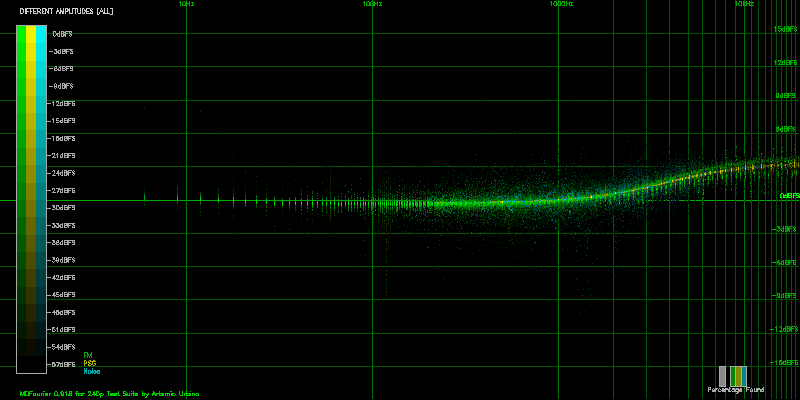
\includegraphics[width=1.0\linewidth]{images/heat/0-plotheat.png}
	\caption[Heat Difference]{Audio difference caused by heat in \textit{Model 1 VA3 system}}
	\label{fig:heatdiff}
\end{figure}

After analysis, it was found that the difference was present only in the left channel and was caused by a severe difference in temperature while recording. The room was at $29^\circ$C\footnote{$84.2^\circ$F} as shown in figure \ref{fig:heatroomtemp}, and the \textit{Sega Genesis Model 1 VA3} under testing had been powered on for around 30 minutes.

\begin{figure}[H]
	\centering
	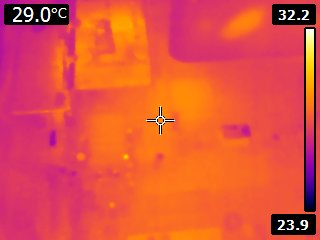
\includegraphics[width=0.4\linewidth]{images/heat/1-roomtemp.jpg}
	\caption[Room temperature]{Console at room temperature \textit{Model 1 VA3 system}}
	\label{fig:heatroomtemp}
\end{figure}

At first warm up differences were suspected, but after some cooling, \textit{cold boot}\footnote{Powering on the console after it had cool down, and immediately making the recording.} and measurements using a thermal camera it was determine that the room temperature on top of the warm up was the culprit, since the results could not be replicated when the room had cooled down to $22^\circ$C\footnote{$71.6^\circ$F}. 

In order to replicate the results, its vents were obstructed to prevent heat dissipation\footnote{Ventilation were covered with electrical tape} for a brief period. The results could be replicated at will under these conditions after just a few minutes of use.

It must be noted that the temperature of the headphone amplifier\footnote{CXA1034} of the console reaches $82.9^\circ$C\footnote{$181.22^\circ$F} with cover removed as shown in figure \ref{fig:heathigh}, so higher temperatures are expected with it closed. This is important since some of the stock capacitors around the headphone amplifier are radiated due to proximity, and can probably reach temperatures beyond their intended rating in warm climates.

\begin{figure}[H]
	\centering
	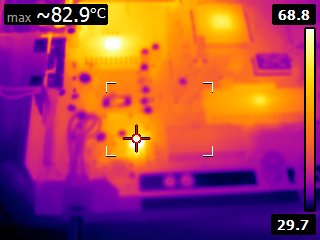
\includegraphics[width=0.4\linewidth]{images/heat/2-hot.jpg}
	\caption[Hot Console]{\textit{Model 1 VA3 system} with amp at $80^\circ$C}
	\label{fig:heathigh}
\end{figure}

\chapter{Requirements}
\label{requirements}
\section{Audio capture device}
\label{audiocards}
For capturing the audio files, an audio capture device is needed. It is recommended to use a musical grade audio card in order to get a flat frequency response across the human hearing spectrum.

So far two audio cards have been used in my personal setup. The reference recordings available for download were made with both cards, a set with each one of them.

I have no association or business relationship with these products, they are just presented as the references used. As more people use the software and we as a community compare files, this list can be expanded with recommendations.

\begin{itemize}
	\item \textbf{M-Audio Audiophile 192:} An internal audio card that is no longer available in the market \cite{maudio}
	\item \textbf{M-Audio M-Track:} A USB audio card. \cite{maudiomtrack}
	\item \textbf{Lexicon Alpha:} An affordable USB audio card. \cite{lexicon}
\end{itemize}

We have tested some cards that don't have a flat frequency response, you should try to use a sound card that is aimed to musicians or instrument recording.

Sound cards have their own sampling internal clock, which tends to deviate enough that frame rate differences can be detected by \textit{MDFourier}. This is compensated for in the time domain while trimming, and it shouldn't be a problem in the frequency domain due to the small variation. \cite{SoundCardClock}

\section{Computer}

Any computer can be used if you are compiling the source code from scratch \cite{sourcecode}, but a statically linked \textit{Microsoft Windows executable} is provided for convinience, alongside a front end. See chapter \ref{usinggui} for instructions on using the GUI.

\section{Game Consoles or emulators}

You'll need either the provided example audio files or create your own by recording from the desired source, which makes more sense since you probably want to compare how these behave.

\section{Flash cart, or means to run the binary}

The console needs to run a custom built binary, a ROM. I will build this functionality into each version of the \textit{240 test suite} \cite{240pSuite} as possible.

In order to run these, you'll either need a flash cart or a custom loading solution compatible with the target platform.

\section{Cables and adapters}

You'll need cables and maybe some adapters to connect the audio output fomr the console to the input of your audio capture card.

\section{Audio capture software}

Your capture card will probably be bundled with some audio editing software, or you can use  Audacity \cite{audacity} or Goldwave \cite{goldwave} options depending on your operating system.

\chapter{Compiling from source code}

Full source code is available for download at \url{https://github.com/ArtemioUrbina/MDFourier/}

\section{Dependencies}

\textit{MDFourier} needs a few libraries to be compiled. In \textit{Linux}, \textit{UN*X} based systems and Cygwin \cite{cygwin}; you can link it against the latest versions of the libraries. 

\begin{itemize}
	\item Fastest Fourier Transform in the West (fftw) \cite{fftw}
	\item The GNU plotutils package \cite{libplot}
	\item PNG Reference Library: libpng \cite{libpng}
	\item Incomplete Beta Function \cite{betafunction} (included with source code)
\end{itemize}

The pre-compiled binary for \textit{Windows} is created with \textit{MinGW}\cite{mingw} and statically linked for distribution against:

\begin{itemize}
	\item fftw-3.3.8 \cite{fftw}
	\item plotutils-2.6 \cite{libplot}
	\item libpng-1.5.30 \footnote{This older version was used to simplify the build process in this statically linked executable. Sources at \url{https://sourceforge.net/projects/libpng/files/libpng15/1.5.30/}}
	\item incbeta \cite{betafunction} (included with source code)
\end{itemize}

The \textit{makefiles} to compile either version are provided with the source code \cite{sourcecode}.

\chapter{Colors available for plots}
\label{availablecolors}

This is the list of colors that can be used in the \textit{MFN configuration file} described in section \ref{mfnconfig}: 

\textit{red, green, blue, yellow, magenta, aquamarine, orange}, and \textit{purple}.

\chapter{Contact the author}
\label{contact}

You can contact me via twitter \url{http://twitter.com/Artemio} or e-mail me at \textit{aurbina@junkerhq.net}.

\chapter{Acknowledgements}

I'd like to thank the following people for helping me so these tools could be completed. First and foremost to my family, who helped me find the time to learn and make progress.

\end{appendices}

\begin{thebibliography}{9}
	\bibitem{FourierTransformApps}
	Bracewell, Ronald N. 
	\textit{The Fourier Transform and Its Applications (2 ed.).}
	McGraw-Hill. ISBN 978-0-07303938-1.
	
	\bibitem{genesisaudio}
	Ace, \textit{GUIDE: A complete overview of the many Sega Genesis/MegaDrive models}
	\url{http://www.sega-16.com/forum/showthread.php?7796-GUIDE-Telling-apart-good-Genesis-1s-and-Genesis-2s-from-bad-ones}
	
	\bibitem{sourcecode}
	Github,
	\textit{MDFourier source code C99},
	\url{https://github.com/ArtemioUrbina/MDFourier/}.
	
	\bibitem{240pSuite}
	240p test Suite,
	\textit{Wiki web page},
	\url{http://junkerhq.net/240p/}.
	
	\bibitem{fftw}
	Fastest Fourier Transform in the West.,
	\textit{web page},
	\url{http://fftw.org/}.
	
	\bibitem{windowtypes}
	Window Types: Hanning, Flattop, Uniform, Tukey, and Exponential ,
	\textit{web page},
	\url{https://community.plm.automation.siemens.com/t5/Testing-Knowledge-Base/Window-Types-Hanning-Flattop-Uniform-Tukey-and-Exponential/ta-p/445063/}.
	
	\bibitem{dbfs}
	dB Full Scale, 
	\url{https://www.sweetwater.com/insync/dbfs/}
	
	\bibitem{SoundCardClock}
	Sound Card Sampling clock variation
	\url{http://www.stu2.net/wiki/index.php/Calibrate_Sound_Card/}
	
	\bibitem{soundcardtiming}
	So how accurate is a typical PC sound card? How stable is the output? How would one measure this?
	Experiments with a PC sound card by leapsecond
	\url{http://www.leapsecond.com/pages/sound-1pps/}
	
	\bibitem{gwsoundcardtiming}
	Each sound card has it's own sampling clock, Goldwave support forums
	\url{http://www.goldwave.ca/forums/viewtopic.php?p=17470}
	
	\bibitem{MontyMontgomery}
	D/A and A/D | Digital Show and Tell (Monty Montgomery @ xiph.org)
	\url{https://www.youtube.com/watch?v=cIQ9IXSUzuM}
	
	\bibitem{leakage}
	Harris, Fredric j. (Jan 1978). \textit{"On the use of Windows for Harmonic Analysis with the Discrete Fourier Transform"}. Proceedings of the IEEE. 66 (1): 51–83.
	\url{https://web.mit.edu/xiphmont/Public/windows.pdf}
	
	\bibitem{zeropaddinginterpolate}
	Spectral Leakage and Zero-Padding of the Discrete Fourier Transform
	\url{https://dspillustrations.com/pages/posts/misc/spectral-leakage-zero-padding-and-frequency-resolution.html}
	
	\bibitem{ZeroPaddingBad}
	Why is it a bad idea to filter by zeroing out FFT bins?
	\url{https://dsp.stackexchange.com/questions/6220/why-is-it-a-bad-idea-to-filter-by-zeroing-out-fft-bins}
	
	\bibitem{libpng}
	libPNG
	\textit{web page},
	\url{https://libpng.sourceforge.io/}
	
	\bibitem{libplot}
	GNU Plot Utils
	\textit{web page},
	\url{https://www.gnu.org/software/plotutils/}
	
	\bibitem{mingw}
	MinGW, 
	\textit{Minimalist GNU for Windows},
	\url{http://mingw.org/}.
	
	\bibitem{cygwin}
	Cygwin,
	\textit{a large collection of GNU and Open Source tools which provide functionality similar to a Linux distribution on Windows.}
	\url{https://www.cygwin.com/}
	
	\bibitem{tukey}
	Tukey window, Recording Blogs
	\url{https://www.recordingblogs.com/wiki/tukey-window}
	
	\bibitem{betafunction}
	incbeta, 
	\textit{Incomplete Beta Function in C},
	\url{https://codeplea.com/incomplete-beta-function-c/}.
	
	\bibitem{maudio}
	M-Audio Audiophile 192,
	\textit{Specifications},
	\url{https://www.soundonsound.com/reviews/m-audio-audiophile-192/}.
	
	\bibitem{lexicon}
	Lexicon Alpha USB card,
	\textit{Product web page},
	\url{https://lexiconpro.com/en/products/alpha/}.
	
	\bibitem{maudiomtrack}
	M-Audio M-Track USB card,
	\textit{Product web page},
	\url{	https://www.m-audio.com/products/view/m-track}.
	
	\bibitem{audacity}
	Audacity
	\textit{web page},
	\url{https://www.audacityteam.org/}.
	
	\bibitem{goldwave}
	Goldwave
	\textit{product web page},
	\url{https://www.goldwave.com/}.
	
	\bibitem{sma}
	Adam Hayes, Simple Moving Average - SMA Definition
	\url{https://www.investopedia.com/terms/s/sma.asp}
\end{thebibliography}

\printglossaries

\end{document}
